\documentclass[../poma-notes.tex]{subfiles}

\begin{document}

\subsection*{Cauchy Sequences}

\begin{definition}
  A sequence $\{p_n\}$ in a metric space $X$ is said to be a \textit{Cauchy} sequence if for every $\epsilon > 0$
  there is an integer $N$ such that $d(p_n, p_m) < \epsilon$ if $n \ge N$ and $m \ge N$.
\end{definition}

\begin{anote}
  度量空间 $X$ 中的序列 $\{p_n\}$ 叫做 \textbf{柯西序列 Cauchy},如果对于任何 $\epsilon > 0$ 存在正整数 $N$,
  只要 $m, n \ge N$ 就有 $d(p_n,p_m) < \epsilon$。根据 Wikipedia:
  \begin{figure}[h]
    \centering
    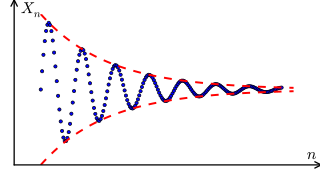
\includegraphics[width=0.5\textwidth]{\subfix{../images/Cauchy_sequence.png}}\par
    一个柯西序列 $\{x_n\}$ 相对于 $n$ 的绘图(蓝色)。如果包含这个序列的空间是完备的,则这个序列的有一个极限。
  \end{figure}

  \begin{figure}[h]
    \centering
    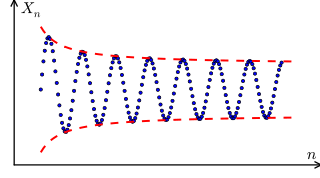
\includegraphics[width=0.5\textwidth]{\subfix{../images/Non_Cauchy_sequence.png}}\par
    一个非柯西序列。这个序列的元素不能随着序列前进而相互靠近。
  \end{figure}
\end{anote}

\begin{definition}
  Let $E$ be a nonempty subset of a metric space $X$, and let $S$ be the set of all real numbers of the form $d(p,q)$,
  with $p \in E$ and $q \in E$. The sup of $S$ is called the \textit{diameter} of $E$.
\end{definition}

如果 $\{p_n\}$ 是 $X$ 中的一个序列,且如果 $E_n$ 包含所有点 $p_N, p_{N+1}, p_{N+2}, \dots$,那么从前两个定义中可以清楚的得到
$\{p_n\}$ 是一个\textbf{柯西序列} 当且仅当
\[\lim_{N \to \infty} diam\ E_N = 0\]

\anote 设 $E$ 是度量空间 $X$ 中的非空子集,又设 $S$ 是一切形式为 $d(p,q)$ 的实数集,$p,q \in E$。$\sup S$ 叫做 $E$ 的直径,
记为 $diam\ E$。

\begin{theorem}\mbox{}
  \begin{enumerate}[label=(\alph*)]
    \item If $\overline{E}$ is the closure of a set $E$ in a metric space $X$, then
          \[diam\ \overline{E} = diam\ E.\]
    \item If $K_n$ is a sequence of compact sets in $X$ such that $K_n \supset K_{n+1} (n=1,2,3,\dots)$ and if
          \[\lim_{n \to \infty} diam\ K_n = 0,\]
          then $\bigcap_1^{\infty} K_n$ consists of exactly one point.
  \end{enumerate}
\end{theorem}

\begin{proof}
  \begin{enumerate}[label=(\alph*)]
    \item 因为 $E \subset \overline{E}$,那么可以清楚的知道
          \[diam\ E \le diam\ \overline{E}\]

          选取 $\epsilon > 0$,$p \in \overline{E}, q \in \overline{E}$。根据 $\overline{E}$ 的定义,$E$ 中存在点 $p'$,$q‘$,
          满足 $d(p,p') < \epsilon,\ d(q,q') < \epsilon$。因此
          \begin{align*}
            \mathcal{} d(p,q) & \le d(p,p') + d(p',q') + d(q',q) \\
                              & < 2\epsilon + d(p',q')           \\
                              & \le 2\epsilon + diam\ E.
          \end{align*}
          它遵循
          \[diam\ \overline{E} \le 2\epsilon + diam\ E,\]
          且因为 $\epsilon$ 是随机的,(a) 则被证明。
    \item 令 $K = \bigcap_1^{\infty} K_n$。根据 Theorem 2.36,$K$ 为非空。如果 $K$ 包含一个以上的点,那么 $diam\ K > 0$。
          但是对于每个 $n$ 而言,$K_n \supset K$,所以 $diam\ K_n \ge diam\ K$。这与假设的 $diam\ K_n \to 0$ 相悖。
  \end{enumerate}
\end{proof}

\begin{anote}
  \begin{enumerate*}[label=(\alph*)]
    \item 如果 $E$ 是度量空间 $X$ 中的集,那么闭包满足 $diam\ \overline{E} = diam\ E$;
    \item 如果 $\{K_n\}$ 是 $X$ 中的紧集的序列,且 $K_n \supset K_{n+1}$ 又若 $\lim_{n \to \infty} diam\ K_n = 0$,
          那么 $\bigcap_1^{\infty} K_n$ 由一个点组成。
  \end{enumerate*}
\end{anote}

\begin{theorem}\mbox{}
  \begin{enumerate}
    \item In any metric space $X$, every convergent sequence is a Cauchy sequence.
    \item In $X$ is a compact metric space and if $\{p_n\}$ is a Cauchy sequence in $X$, then $\{p_n\}$ converges to
          some point of $X$.
    \item In $R^k$, every Cauchy sequence converges.
  \end{enumerate}
\end{theorem}

注意:收敛的定义与柯西序列定义的不同在于前者明确存在极限,后者未必。因此 Theorem 3.11(b) 可以判定一个序列是否收敛,而不需知道其收敛的极限。
事实(包含于 Theorem 3.11)上,一个序列收敛在 $R^k$,当且仅当它是一个柯西序列,这通常被称为收敛的\textbf{柯西标准}。

\begin{proof}
  \begin{enumerate}[label=(\alph*)]
    \item 如果 $p_n \to p$ 且 $\epsilon > 0$,存在一个整数 $N$ 对于所有的 $n \ge N$ 满足 $d(p,p_n) < \epsilon$。因此
          只要 $n \ge N$ 同时 $m \ge N$,那么
          \[ d(p_n, p_m) \le d(p_n, p) + d(p, p_m) < 2\epsilon \]
          因此 $\{p_n\}$ 是一个柯西序列。
    \item 令 $\{p_n\}$ 为一个在紧空间 $x$ 的柯西序列。对于 $N=1,2,3,\dots$,令 $E_N$ 为一个包含了 $P_N,P_{N+1},P_{N+3},\dots$
          的集合。那么根据 Definition 3.9 与 Theorem 3.10(a),有
          \begin{equation}
            \lim_{N \to \infty} diam\ \overline{E}_N = 0
          \end{equation}
          作为紧空间 $X$ 中的一个闭集,每个 $\overline{E}_N$ 都是紧的(Theorem 2.35)。又因为 $E_N \supset E_{N+1}$,因此有
          $\overline{E}_N \supset \overline{E}_{N+1}$。

          Theorem 3.10(b) 说明存在一个唯一的 $p \in X$ 位于每个 $\overline{E}_N$ 中。

          令 $\epsilon > 0$,根据 (3) 存在一个整数 $N_0$ 当 $N \ge N_0$时,满足 $\overline{E}_N < \epsilon$。又因为
          $p \in \overline{E}_N$,对于每个 $q \in \overline{E}_N$ 它遵循 $d(p,q) < \epsilon$,所以对于每个 $q \in E_n$
          也成立。换言之,如果 $n \ge N_0$,那么就有 $d(p,p_n)<\epsilon$。即 $p_n \to p$。
    \item 令 $\{\mathbf{x}_n\}$ 为一个在 $R^k$ 上的柯西序列。如同 (b) 那样定义 $E_N$,用 $\mathbf{x}_i$ 替换 $p_i$。对于某些
          $N$ 而言,$diam\ E_N<1$。$\{\mathbf{x}_n\}$ 的值域是 $E_N$ 与有限集 $\{\mathbf{x}_1,\dots,\mathbf{x}_{N-1}\}$
          的并集。因此 $\{\mathbf{x}_n\}$ 是有界的。因为每个 $R^k$ 的有界子集在 $R^k$ 中拥有紧闭包(Theorem 2.41),(c) 遵循了
          (b)。
  \end{enumerate}
\end{proof}

\begin{definition}
  A metric space in which every Cauchy sequence converges is said to be \textbf{complete}.
\end{definition}

因此 Theorem 3.11 说的\textit{所有紧度量空间以及所有欧几里得空间是完备的}。Theorem 3.11 同样说明了\textit{一个完备度量空间 $X$ 中的
  每个闭子集 $E$ 都是完备的}。(每个在 $E$ 中的柯西序列也是 $X$ 中的柯西序列,因此它收敛于某 $p \in X$,且实际上 $p \in E$,因为 $E$
是闭的)。一个度量空间中不具完备性质的例子是,所有符合 $d(x,y) = |x - y|$ 的有理数。

Theorem 3.2(c) 与 Definition 3.1 中的 example(d) 说明了收敛的序列是有界的,而在 $R^k$ 上有界的序列并不需要收敛。不过这里有一个重要
的例子,收敛等同于有界;这发生在 $R^1$ 中的单调序列。

\begin{definition}
  A sequence $\{s_n\}$ of real numbers is said to be
  \begin{enumerate}[label=(\alph*)]
    \item \textit{monotonically increasing} if $s_n \le s_{n+1} (n=1,2,3,\dots)$;
    \item \textit{monotonically decreasing} if $s_n \ge s_{n+1} (n=1,2,3,\dots)$;
  \end{enumerate}
\end{definition}

单调序列的类由递增以及递减序列所构成。

\anote 实数序列的\textbf{单调递增}($s_n \le s_{n+1}$)和\textbf{单调递减}。

\begin{theorem}
  Suppose $\{s_n\}$ is monotonic. Then $\{s_n\}$ converges if and only if it is bounded.
\end{theorem}

\begin{proof}
  假设 $s_n \le s_{n+1}$(另一方向的证明类似)。令 $E$ 为 $\{s_n\}$ 的值域。如果 $\{s_n\}$ 有界,令 $s$ 为 $E$ 的最小上界。那么有
  \[ s_n \le s \qquad (n=1,2,3,\dots) \]
  对于每个 $\epsilon > 0$,有一个整数 $N$ 满足
  \[ s - \epsilon < s_N \le s \]
  否则 $s - \epsilon$ 将会变为 $E$ 的一个上界。由于 $\{s_n\}$ 递增,$n \ge N$ 因此说明
  \[ s - \epsilon < s_n \le s \]
  即 $\{s_n\}$ 收敛(于 $s$)。

  另一方向的证明遵从 Theorem 3.2(c)。
\end{proof}

\anote 单调序列收敛,当且仅当它是有界的。

\end{document}
